\chapter{Elasticities}

\section{The Elasticity of Demand}



\subsection{The Price Elasticity of Demand}

\begin{itemize}

	\item A good's \underline{price elasticity of demand} measures how much the quantity demanded responds to a change in price.
	
	\item Demand for a good is \underline{elastic} if the quantity demanded responds a lot to changes in price.
	
	\item Demand is \underline{inelastic} if the quantity demanded doesn't respond a lot to changes in price. 

\end{itemize}

\underline{Determinants of Price Elasticity of Demand}

\begin{enumerate}

	\item Availability of Substitutes: Goods with close substitutes are more elastic.
		
	\item Necessities v. Luxuries: Necessities are more inelastic and luxuries are more elastic.
	
	\item Market Definition: Goods in narrowly defined markets are more elastic, and goods in broadly defined markets are more inelastic.
	
%		\begin{itemize}
%		
%		\item Ex. Vanilla ice cream is a narrowly defined good, so it has lots of substitutes.
%		
%		\item Ex. Food is a broadly defined good, so it has no substitutes.
%		
%		\end{itemize}
		
	\item Time Horizon: Goods are more elastic in the long term than the short term.
	
%		\begin{itemize}
%		
%		\item Ex. In the short run, demand for gasoline is inelastic because most people can't readily change their commute.
%		
%		\item Ex. In the long run, demand for gasoline is elastic because people buy more fuel-efficient cars, switch to public transportation, or move closer to work. 
%		
%		\end{itemize}

\end{enumerate}



\subsection{Computing the Price Elasticity of Demand}

\begin{itemize}

	\item Price elasticity of demand is
	
		 \[ \eta = \left| \frac{\% \Delta Q_D}{\% \Delta P} \right| \]
	 
	 \item Ex. The price of ice-cream increases by 10\%, and the quantity bought decreases by 20\%. The price elasticity of demand is:
	 	\[ \eta = \left| \frac{-20\%}{10\%} \right| = 2 \]

\end{itemize}



\subsection{The Midpoint Method}

\begin{itemize}

	\item Problem: The typical percent change calculation depends on the initial point.
	
	\item Ex.
		\begin{gather*}
		Point \ A: \ P_A = \$4, \ Q_A = 120 \\
		Point \ B: \ P_B = \$6, \ Q_B = 80
		\end{gather*}
		\begin{gather*}
		\% \Delta P_{A \rightarrow B} = \frac{P_B - P_A}{P_A} = \frac{6 - 4}{4} = \frac{1}{2} \\
		\% \Delta P_{B \rightarrow A} = \frac{P_A - P_B}{P_B} = \frac{4 - 6}{6} = -\frac{1}{3}
		\end{gather*}
	
	\item Solution: The \underline{midpoint method} calculates percent change by using the midpoint of the two values in the denominator. 
	
	\item Ex. \[ \% \Delta P = \frac{P_B - P_A}{\frac{P_A + P_B}{2}} = \frac{6 - 4}{\frac{4 + 6}{2}}  = \frac{2}{5} = 40\% \]
	
	\item To calculate elasticities, use the midpoint method.
	
	\item Ex. 
	\begin{gather*}
	\eta = \left| \frac{\% \Delta Q}{\% \Delta P} \right| \\
	\% \Delta Q = \frac{Q_A - Q_B}{\frac{Q_A + Q_B}{2}} = \frac{120 - 80}{\frac{120 + 80}{2}} = \frac{2}{5} \\
	\% \Delta P = \frac{P_A - P_B}{\frac{P_A + P_B}{2}} = \frac{4 - 6}{\frac{4 + 6}{2}} = -\frac{2}{5} \\
	\eta = 1
	\end{gather*}
		
\end{itemize}



\subsection{Classifying Demand Curves}

\begin{itemize}

\item Demand is \underline{elastic} when the elasticity is greater than 1.

\item Demand is \underline{inelastic} when the elasticity is less than 1.

\item Demand is \underline{unit elastic} when the elasticity equals 1.

\item The flatter a demand curve is, the more elastic it is.

\begin{figure}[h]
Elasticity of Demand Curves
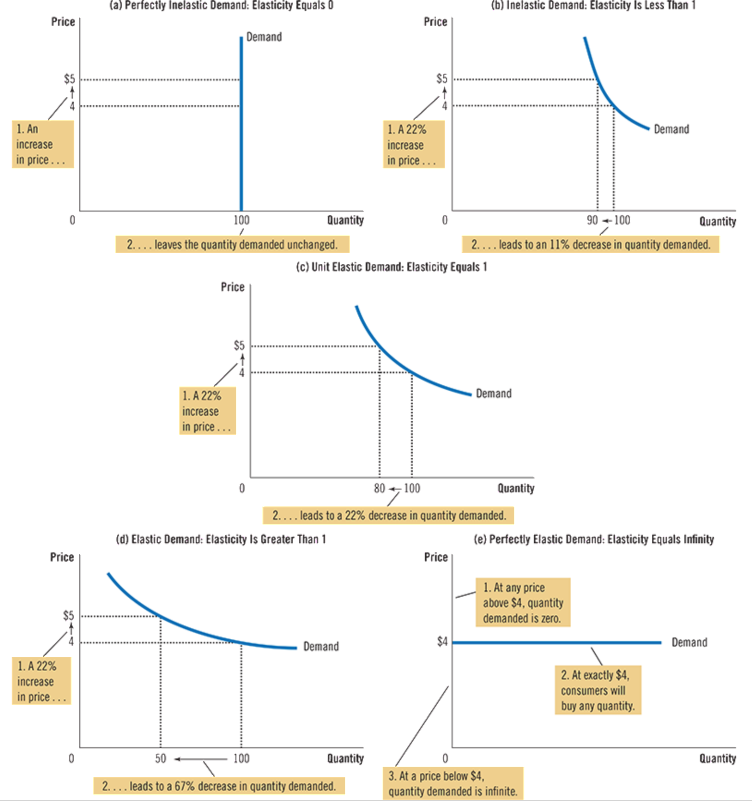
\includegraphics[width = \textwidth]{2.1.4_elasticity_of_d}
\centering
\end{figure}

\end{itemize}



\subsection{Total Revenue and Price Elasticity of Demand}

\begin{itemize}

\item \underline{Total Revenue} in a market is the amount paid by buyers and received by sellers.

\item Algebraically, \[TR = P \times Q\]

\newpage

\item Graphically, 

\begin{figure}[h]
Total Revenue
\centering
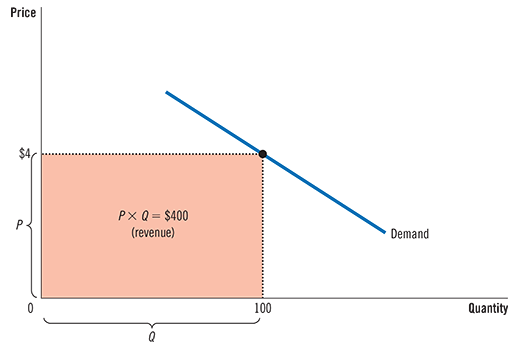
\includegraphics[width = \textwidth]{2.1.5_total_rev}
\end{figure}

\item The price elasticity of demand determines how a price change affects total revenue


\item If demand is inelastic, an increase in price increases total revenue

\item If demand is elastic, an increase in price decreases total revenue

\begin{figure}[h]
Total Revenue and Elasticity
\centering
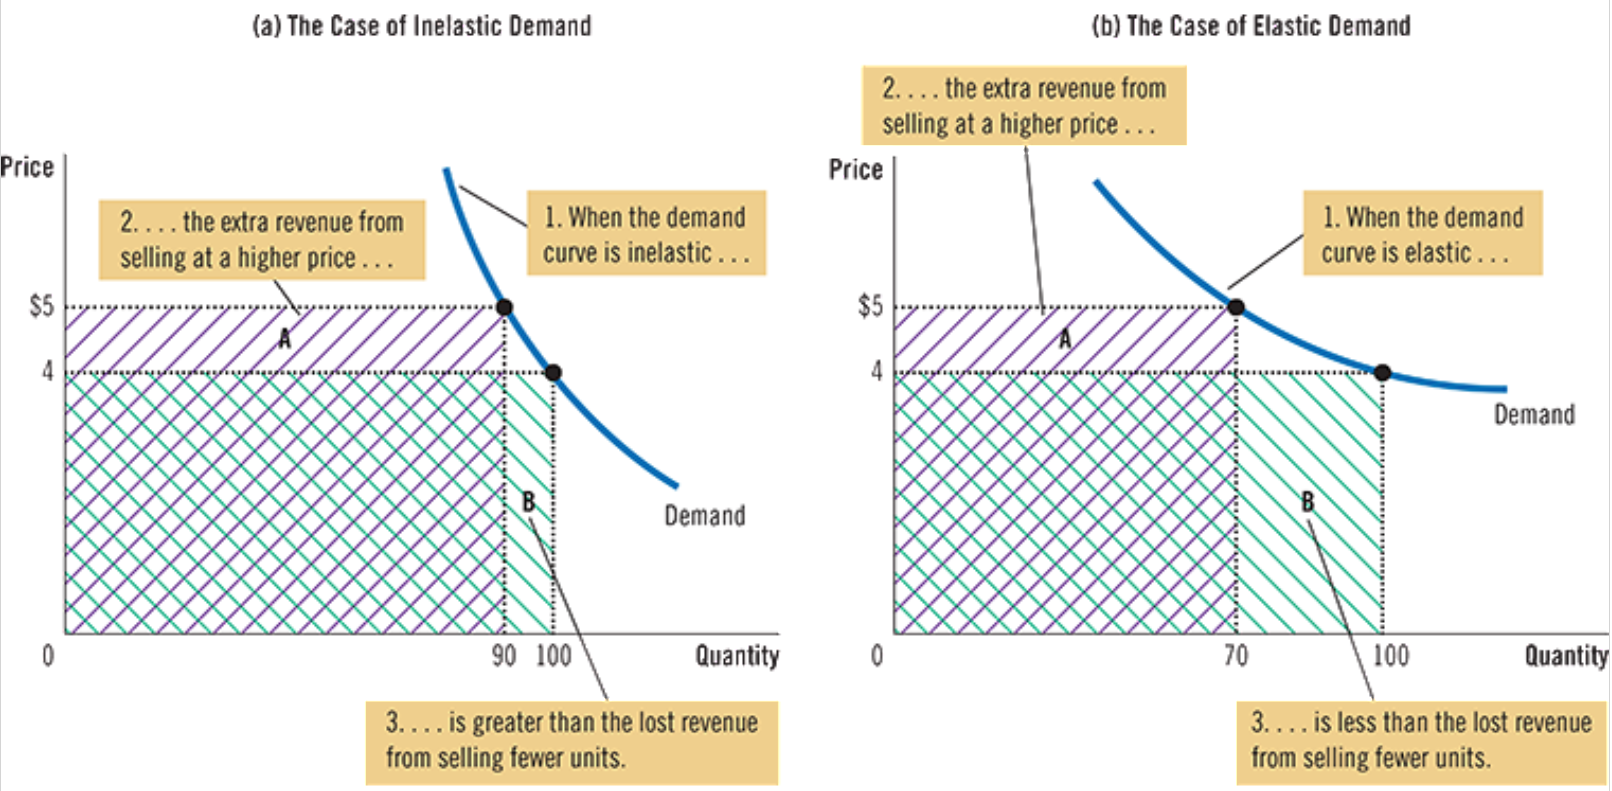
\includegraphics[width = 0.9\textwidth]{2.1.5_tr_elasticity}
\end{figure}

\end{itemize}

\newpage



\subsection{Price Elasticity of Demand for Linear Demand Curves}

\begin{itemize}

\item The elasticity of linear demand curves is non-constant

\begin{figure}[h]
\centering
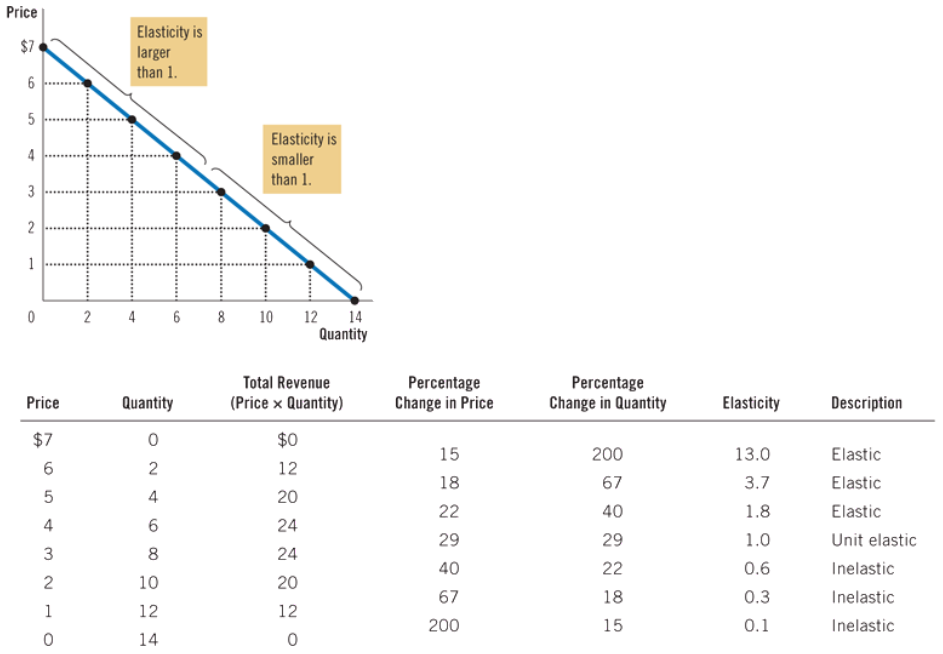
\includegraphics[width = \textwidth]{2.1.6_elasticity_linear_d}
\end{figure}

\end{itemize}



\subsection{Other Demand Elasticities}

\begin{itemize}

\item The \underline{income elasticity of demand} measures how the quantity demanded changes as consumer income changes.
	\[\text{Income elasticity of demand} = \frac{\% \Delta Q_D}{\% \Delta I} \]
	
	\begin{itemize}
	
	\item Normal goods have positive income elasticities of demand.
	
	\item Inferior goods have negative income elasticities of demand.
	
	\end{itemize}
	
\item The \underline{cross-price elasticity of demand} measures how the quantity demanded of one good responds to a change in the price of another good.
	\[ \text{Cross-price elasticity of demand} = \frac{\% \Delta Q_{D,X}}{\% \Delta P_Y} \]
	
	\begin{itemize}
	
	\item Substitutes have positive cross-price elasticities of demand.
	
	\item Complements have negative cross-price elasticities of demand.
	
	\end{itemize}
	
\end{itemize}